\chapter{Dataset Overview} \label{chap:dataset}

This project relies on the \textit{Olympic Games Medals 1986-2022} dataset, sourced from Kaggle \cite{olympic_19862022}. This dataset was originally scraped from the official International Olympic Committee website \cite{olympics}, ensuring its alignment with authoritative data sources. It consists of multiple files, each providing specific details about athletes, medal outcomes, event results, and hosting nations. Key files include:

\begin{itemize}
    \item \texttt{olympic\_athletes.csv}: Details about athletes, including demographics and participation history.
    \item \texttt{olympic\_medals.csv}: Records of medals awarded across events and disciplines.
    \item \texttt{olympic\_hosts.csv}: Information about hosting cities, countries, and the duration of each Olympic event.
    \item \texttt{olympic\_results.csv}: Comprehensive details on event results, including participants and rankings.
\end{itemize}

Despite its extensive coverage, the raw dataset required significant preprocessing and cleaning to address inconsistencies and prepare it for analysis.

\section{Inconsistent Data Entries}

The raw dataset contained several inconsistencies in data entries that required attention during the preprocessing phase. Two significant issues encountered were duplicate records and invalid birth years. These problems had to be resolved to ensure the dataset's reliability and accuracy for analysis.

\subsection{Duplicate Records}

Duplicate entries for athletes and events were present in the dataset, leading to redundancies and inaccuracies. For instance, multiple records existed for the same athlete across different events or Olympic appearances, making it challenging to analyze unique participation trends. These duplicate entries were systematically identified using key attributes, such as athlete names, event details, and medal information, and subsequently removed to maintain data integrity.

\subsection{Invalid Birth Years}

Another major inconsistency was the presence of invalid or missing birth years for athletes. Implausible values, such as negative birth years or years indicating extreme ages (e.g., over 150 years), were identified in the dataset. These anomalies introduced inaccuracies in calculating athletes' ages at their first Olympic appearance and other related analyses.

To address this, reasonable age boundaries for Olympic participation were established based on historical records. According to sources, the youngest known Olympian was 10 years old \cite{youngest_olympian}, and the oldest recorded Olympian was 73 years old \cite{oldest_olympian}. Using these references, red shaded regions in the visualizations highlight implausible age values falling outside this range.

Figure \ref{fig:birth_years} shows the distribution of athletes' birth years by their first Olympic appearance, with anomalies clearly visible as athletes cannot have their first Olympic appearance before the year their were born. The red shaded region highlights implausible values, including negative ages and values exceeding typical human lifespans. Similarly, Figure \ref{fig:athlete_ages} illustrates the distribution of athletes' ages at their first Olympic appearance.

\begin{figure}[ht]
    \centering
    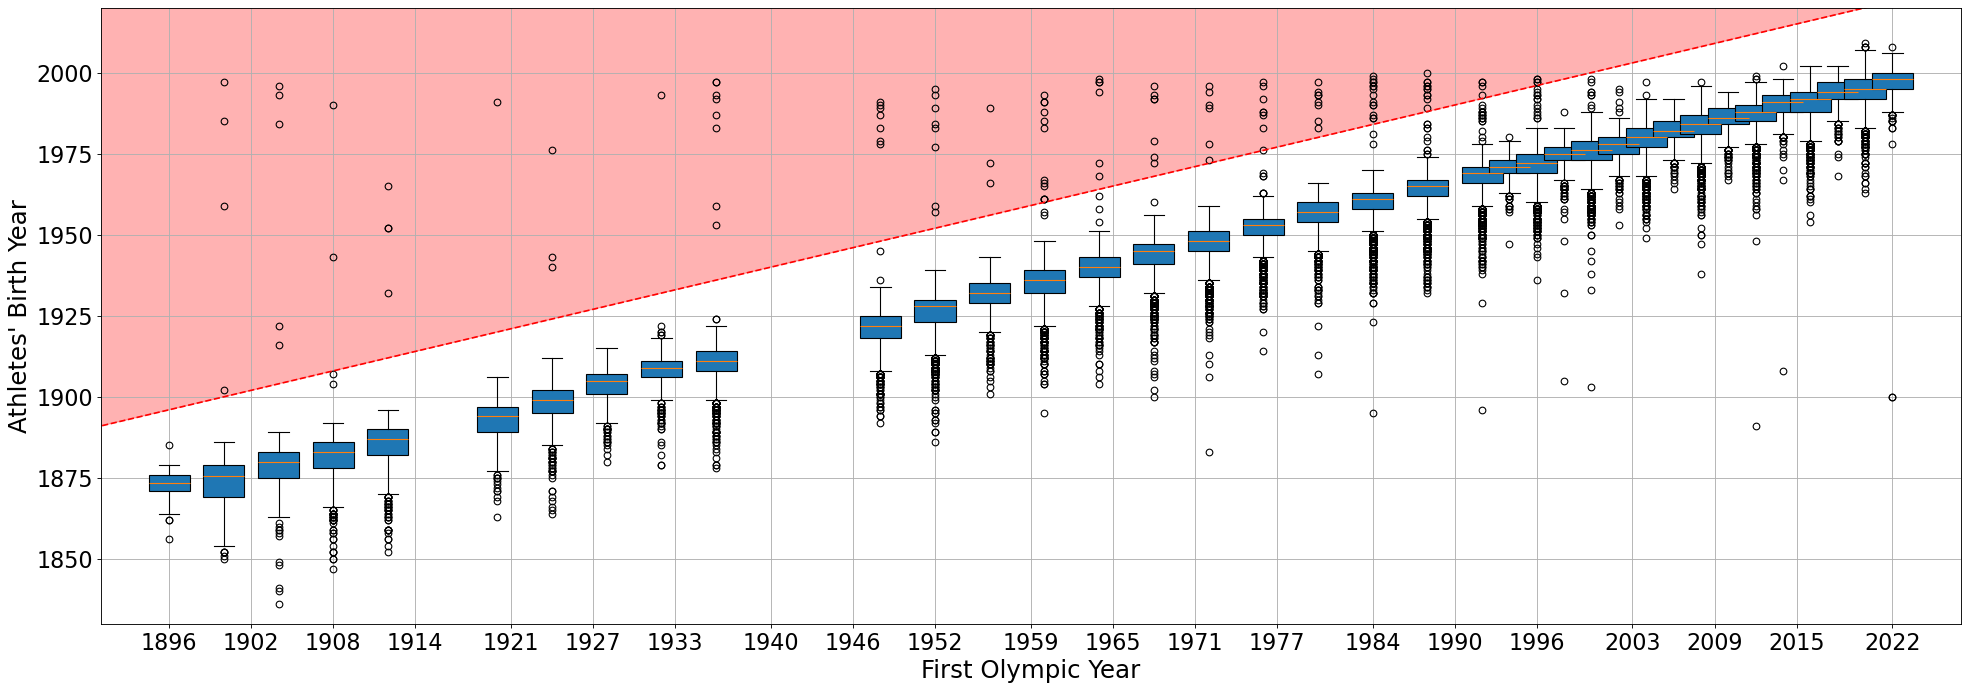
\includegraphics[width=\textwidth, keepaspectratio]{Distribution of Athletes' Birth Years by First Olympic Appearence.png}
    \caption{Distribution of Athletes' Birth Years by First Olympic Appearance}
    \label{fig:birth_years}
\end{figure}

\begin{figure}[ht]
    \centering
    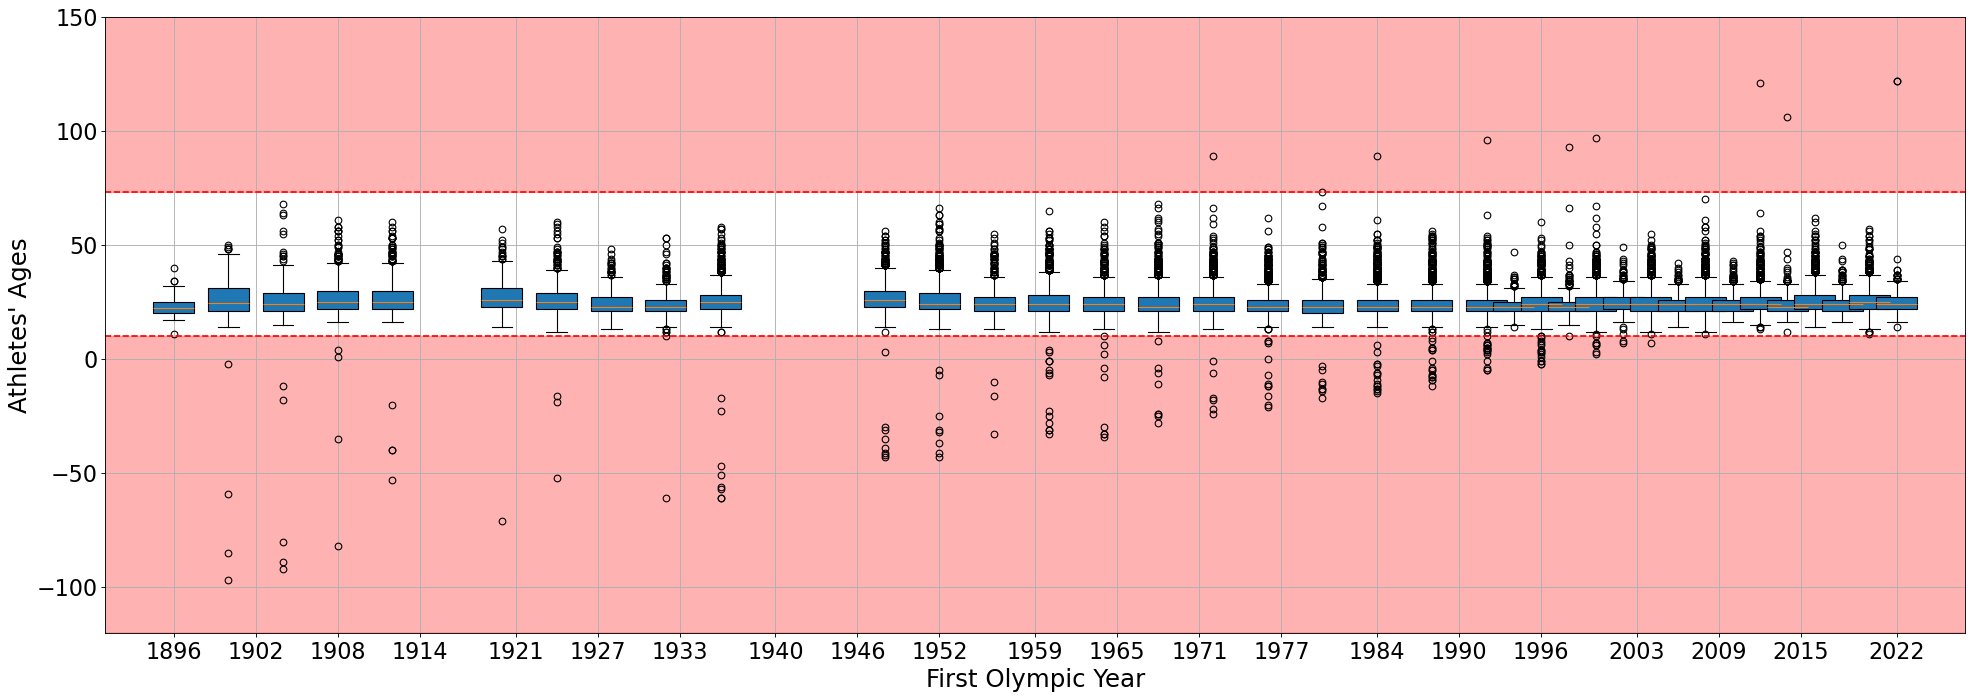
\includegraphics[width=\textwidth, keepaspectratio]{Distribution of Athletes' Ages at Their First Olympic Appearence.png}
    \caption{Distribution of Athletes' Ages at Their First Olympic Appearance}
    \label{fig:athlete_ages}
\end{figure}

\section{Ambiguous Geographical Data}

Geographical data in the raw dataset was often ambiguous or inconsistent. Key issues included:

\begin{itemize}
    \item \textbf{Host City and Country Mapping:} Host cities were inconsistently labeled or lacked corresponding country information. To resolve this, city names were mapped to their respective countries using geocoding tools such as Nominatim \cite{nominatim}.
    \item \textbf{Country Code Discrepancies:} Standardized two-letter (ISO 3166-1 alpha-2) and three-letter (ISO 3166-1 alpha-3) country codes were assigned to all entries to eliminate inconsistencies in naming conventions.
\end{itemize}

By standardizing geographical data, we ensured consistency and improved the dataset's usability for visualizations involving country-specific analyses.


\section{Missing Metadata}

A significant portion of the dataset contained missing or incomplete metadata, particularly for athletes and events. Common issues included:

\begin{itemize}
    \item \textbf{Incomplete Athlete Information:} Some athletes lacked URLs, full names, or demographic details. Such records were filtered out when critical information was unavailable.
    \item \textbf{Unresolved Medalist Metadata:} Certain medalists had incomplete associations with their events or disciplines, which limited their analytical use.
\end{itemize}

These gaps were addressed where possible, and records that could not be resolved were excluded from further analysis.
